%%!TEX TS-program = pdflatexmk
%%!TEX encoding = UTF-8 Unicode
\documentclass[letterpaper,11pt]{article}
\usepackage[utf8]{inputenc}
\usepackage[body={6.0in,9.0in}, vmarginratio=1:1]{geometry}
\usepackage[small,compact]{titlesec}

%\usepackage[expert]{fourier}
\usepackage{fourier}
\usepackage[scaled=0.85]{berasans}
\usepackage[scaled=0.85]{beramono}

\usepackage{booktabs}

% Include graphicx
\usepackage{graphicx}
%\usepackage{applekeys}

\usepackage{microtype}

\usepackage{xcolor}
\usepackage[colorlinks, urlcolor=darkgray, linkcolor=darkgray]{hyperref}

%\newcommand{\MacTeX}{Mac\TeX}
\newcommand{\MacTeX}{Mac\kern-.12em\TeX}
\newcommand{\BibTeX}{B\textsc{i\kern-.025em  b}\kern-.13em\TeX}
\newcommand{\conTeXt}{Con\kern-.12em\TeX t}
\newcommand{\TS}{\textsf{\TeX Shop}}
% default small caps used for utopia are ugly; don't want to use [expert] here.
%\newcommand{\acr}[1]{\textsc{#1}}
%\usepackage{relsize}
%\newcommand{\acr}[1]{\textrm{\smaller\uppercase{#1}}}
\newcommand{\acr}[1]{\textsf{#1}}
%\newcommand{\cmd}[1]{\texttt{#1}}
%\newcommand{\mnu}[1]{\texttt{#1}}
\newcommand{\cmd}[1]{\textsf{#1}}
\newcommand{\mnu}[1]{\textsf{#1}}
\newcommand{\To}{\,\(\to\)\,}

% set | as a command character within verbatim so you can execute commands there
\usepackage{verbatim}
\makeatletter
\addto@hook\every@verbatim{\catcode`|=0}
\makeatother

% define colored items to be inserted in verbatim environments
\setlength{\fboxsep}{0pt}
\newcommand{\selmark}{\colorbox{green}{\rule[-0.5ex]{0ex}{2.1ex}\texttt{•}}}

\title{\TS\ Tips \& Tricks\\\small v0.5.0--2011/04/20}
\author{H. Schulz\\\small\href{mailto:herbs2@mac.com}{herbs2@mac.com}}
\date{}

\begin{document}
\maketitle

\tableofcontents

\newpage

\section{Introduction}

\TS\ is a ``Front End'' for a \TeX\ distribution on Mac OS~X. As such it allows the user to create and edit \TeX\ source files, interact with the \TeX\ distribution (e.g., typeset the source file) and, finally preview the final \acr{pdf} file. It also allows the user to go back and forth between preview and source.

Over the years \TS\ has added many features. Some of them are obvious and are meant to help a novice get started. Others are a bit more subtle in their use and the underlying power of these features needs to be coaxed out.

\subsection{What Isn't Here}

This article is, first of all, \emph{not} about \TeX\ or \LaTeX. I don't intend to teach you how to write \TeX\ source. There are many fine books and articles that will teach you how to become a \TeX pert or, at least, a \TeX pätzer like me.

Although there is some introductory material it is also \emph{not} meant as a complete manual for the use of \TS\ for the total novice. Over time it might evolve into such a document but I've got to start somewhere and this is that start.

\subsection{What Is Here}

In this article I hope to introduce you to some of the more subtle things you can do to make your life as a \TeX\ source editor easier. These include adding keyboard commands and extending the editing capabilities of \TS; helping you make short(er) work of creating documents, etc., with the use of Macros and Command Completion; and, finally, how one can extend the processing capabilities of \TS\ using Engines.

\section{Editing, Typesetting and Viewing --- the Work Cycle}

This is about as close to a beginner's section you will get in this document.

\subsection{Editing the Source File}

The first thing you've got to do to create that great work is to type it into the source document that will be typeset and viewed later. This involves both putting \LaTeX\ markup as well as your wonderful words into the document.

To get started you can open a new document using \mnu{File}\To\mnu{New} (\cmd{Cmd-N}) and then fill in the start of a new document by choosing a template from the \mnu{Templates} popup menu in the Source Window or use---new with \TS\ 2.36---the \mnu{File}\To\mnu{New From Stationery…} command and picking appropriate Stationery from the list. Note that the templates and stationery provided are certainly not complete; if you have some that you think are of general use feel free to submit them for inclusion in \TS. You can add personal Templates and Stationery to \path{~/Library/TeXShop/Templates/} and \path{~/Library/TeXShop/Stationery/} respectively. \textbf{Note: \path{~/Library/} is the \texttt{Library} folder in your \texttt{HOME} folder.}

\subsubsection{\LaTeX\ \& Matrix Panels}

While I believe that panels with a clickable interface actually hinder learning I'll mention that TeXShop has two panels to help with entering \LaTeX\ code (the \LaTeX\ Panel) and for setting up the basic structure of a matrix or tabular (the Matrix Panel). These are toggled on/off under the \mnu{Window} Menu or with the keyboard shortcuts\footnote{The given shortcuts are for the English localization and may be different with other localizations.} \texttt{Opt-Cmd-{}-} and \texttt{Opt-Cmd-=} respectively. Figure (\ref{fig:LandMPanels}) shows what the panels look like.
\begin{figure}
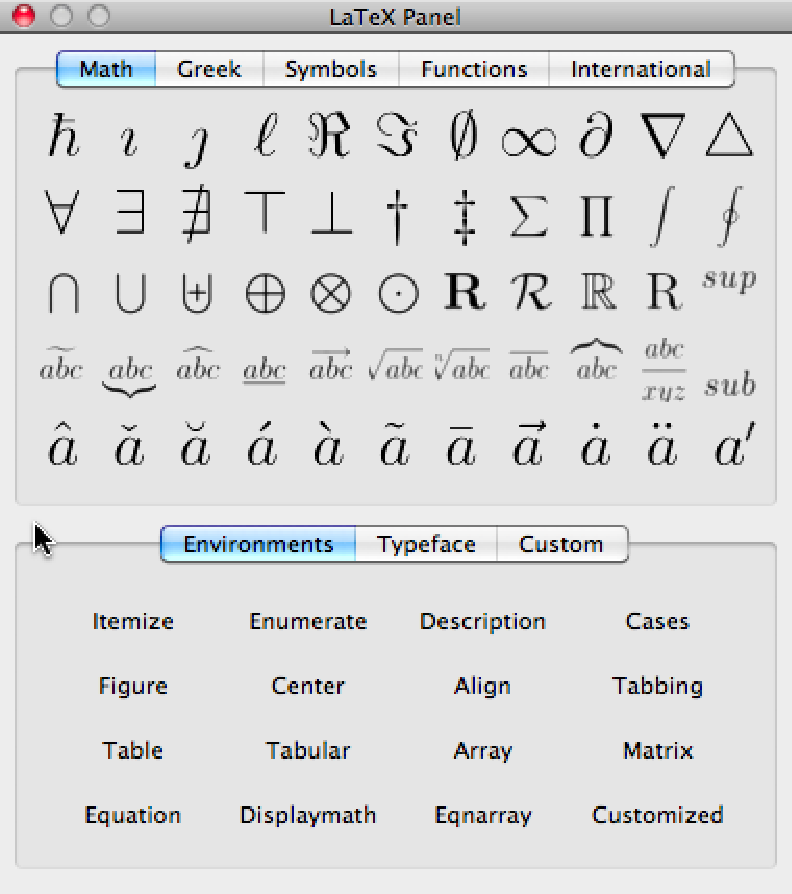
\includegraphics[width=2.5in]{figs/LaTeXPanel}\hfill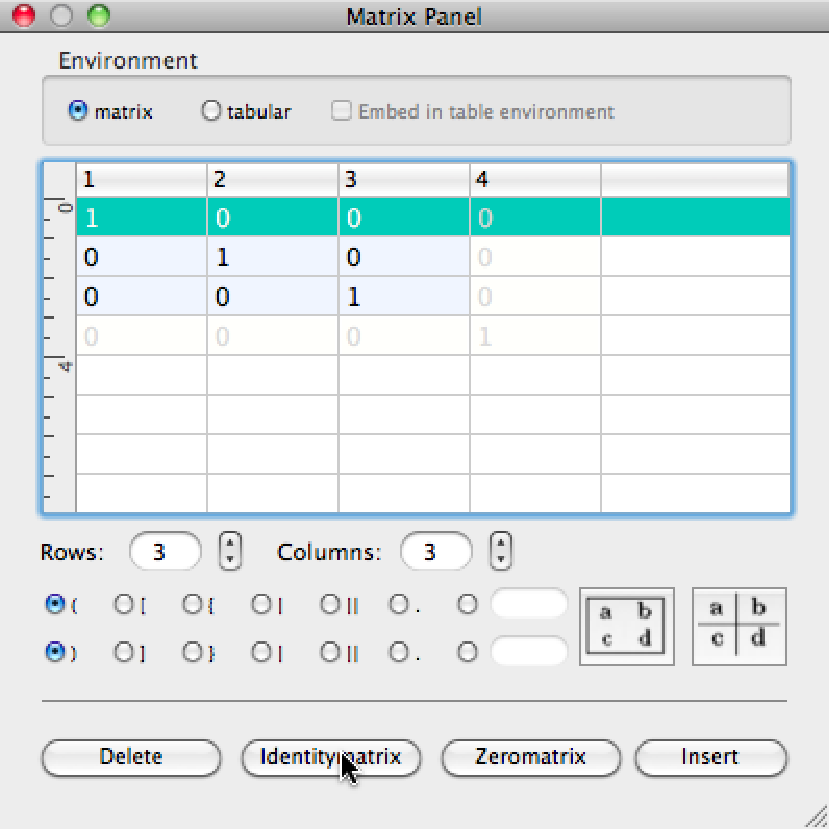
\includegraphics[width=2.5in]
{figs/MatrixPanel}
\caption{The \LaTeX\ \& Matrix Panels.}
\label{fig:LandMPanels}
\end{figure}
It is possible to make a few changes and additions to the \LaTeX\ Panel by editing the 
\path{~/Library/TeXShop/LatexPanel/completion.plist} file. \textbf{Note: all \path{plist} files must be edited using UTF-8 Unicode encoding.}

\subsubsection{The Tags Popup}

The \mnu{Tags} popup menu on the Source Toolbar will automatically list sectioning commands so you can quickly jump to a relevant part of your document source. You can add your own tag to the list at a particular place in the document by placing the line
\begin{verbatim}
%:my tag name
\end{verbatim}
at that position and it will then appear in the popup list so you can jump to that location quickly. See Figure (\ref{fig:Tags}). Sorry, tags are not recursively included for files you \verb|\include| or \verb|\input|.
\begin{figure}
\centering
\framebox{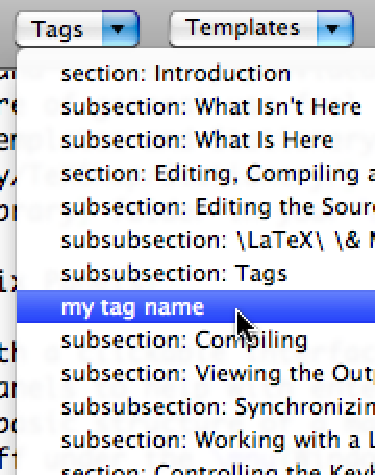
\includegraphics[width=1.5in]{figs/Tags}}
\caption{The Tags Popup Menu.}
\label{fig:Tags}
\end{figure}

\subsection{Typesetting}

Once you are ready to take a look at how your document will appear you typeset it with the default engine, \texttt{pdflatex} out of the box, by simply using the \mnu{Typeset}\To\mnu{Typeset} (\cmd{Cmd-T}) command.

You may wish to use a different engine as your default. You can change the default engine in \mnu{TeXShop}\To\mnu{Preferences}\To\mnu{Typesetting}.

If you are including many \acr{eps} graphics files in your document you may wish to typeset using \texttt{latex}\To\texttt{dvips}\To\texttt{ps2pdf} since \texttt{pdf(la)tex} does not allow for direct inclusion of \acr{eps} files\footnote{The \texttt{pdflatex} program in \MacTeX-2010 and later will do on-the-fly conversion of \acr{eps} files.}. The easiest way to do this is to include the line
\begin{verbatim}
% !TEX TS-program = latex
\end{verbatim}
at the top of your document. Then \TS\ will use the \texttt{latex+distiller} typesetting method noted above no matter what the default engine setting. Change \texttt{latex} to \texttt{pdflatex} to force use of \texttt{pdflatex} to typeset your file.

\subsection{Viewing the Output \acr{pdf} File}

Assuming the document was successfully typeset the \acr{pdf} file will automatically open in a separate preview window.

You can control how it's displayed in the \mnu{Preview} Menu. You can change the default settings in \mnu{TeXShop}\To\mnu{Preferences}\To\mnu{Preview}.

\subsubsection{Synchronizing between \acr{pdf} and Source}

With more recent \TeX\ distributions you can also skip back and forth between a location in the Preview Window and the equivalent location in the Source Window by \cmd{Cmd-Clicking} in either one to go to the (approximate) location in the other. See Figure (\ref{fig:SourcePreviewSync}) for an example of Source\To Preview and Preview\To Source synchronization.

\begin{figure}
\centering
\framebox{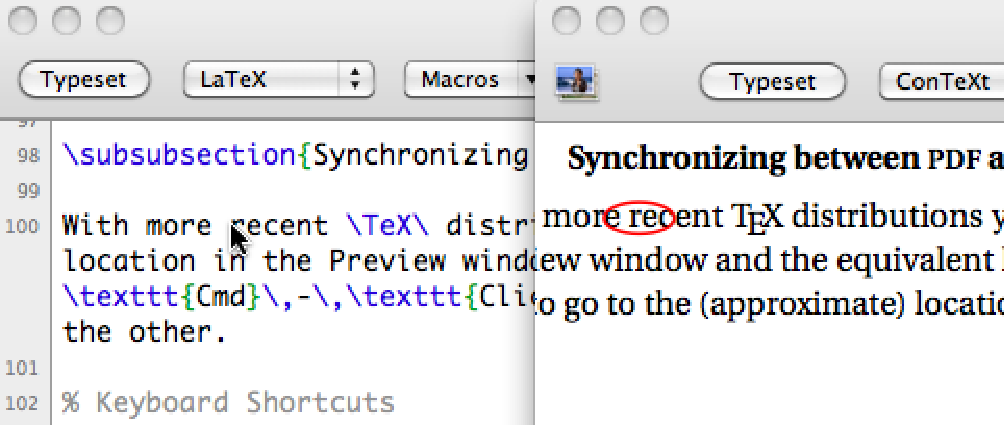
\includegraphics[width=2.75in]{figs/SourceToPreviewSync}}\qquad\framebox{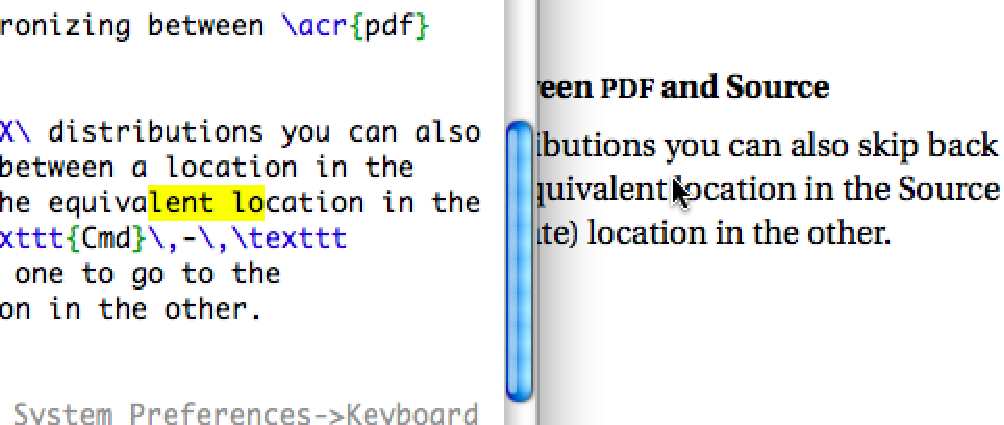
\includegraphics[width=2.75in]{figs/PreviewToSourceSync}}
\caption{Source\To Preview and Preview\To Source Synchronization.}
\label{fig:SourcePreviewSync}
\end{figure}

\subsection{Working with a Large Document}

It is often handy to break a large document into more manageable subordinate parts and then create a ``root'' file which contains the preamble and \verb|\include| commands to bring all the parts together for typesetting.

To have \TS\ ``know'' which file to typeset when working on a subordinate file put the line
\begin{verbatim}
% !TEX root = path/to/rootfile.tex
\end{verbatim}
at the top of your subordinate file; \path{path/to/rootfile.tex} is the relative or absolute path to the root file for this document. Once this is done \TS\ will typeset the root file if you press \mnu{Typeset}\To\mnu{Typeset} (\cmd{Cmd-T}) even though you are editing a subordinate file and properly synchronize between the Source and \acr{pdf}. E.g., if the root file is called \path{mygreatbook.tex} and the chapter files, \path{chapter1.tex}, etc., are in a \path{chapters} sub-folder below the root file then place the line
\begin{verbatim}
% !TEX root = ../mygreatbook.tex
\end{verbatim}
at the top of each of the chapter files. The \path{../} means go up one folder level to find the root file.

\subsubsection{Switching between Source Windows}

If you have multiple source files open you can switch between just those files by using the \mnu{Window}\To\mnu{Next/Previous Source Window} (\cmd{Cmd-F2}/\cmd{Shft-Cmd-F2}) menu commands.

\subsection{Working with \cmd{BibDesk} and Citations}

\TS\ has a built-in ``plugin'' that interacts with the \cmd{BibDesk} bibliography application to allow you to complete citation references in the \verb|\cite| command.  To enable the use of the ``plugin'' make sure that \mnu{TeXShop}\To\mnu{Preferences}\To\mnu{Source}\To\mnu{Editor}\To\mnu{BibDesk Completions} is checked. 

To use it you must first open the required bibliography (\texttt{bib}) file(s) in \cmd{BibDesk}. Enter several characters from the reference label within the \verb|\cite| command and press \cmd{F5} to get a list of matching references from the \texttt{bib} file(s) with a bit of information about each one. Scroll to the one you want and press \cmd{Return} or \cmd{Tab}. See Figure (\ref{fig:bibdesk}) 
on page (\pageref{fig:bibdesk}) for an example.
\begin{figure}
\centering
\fbox{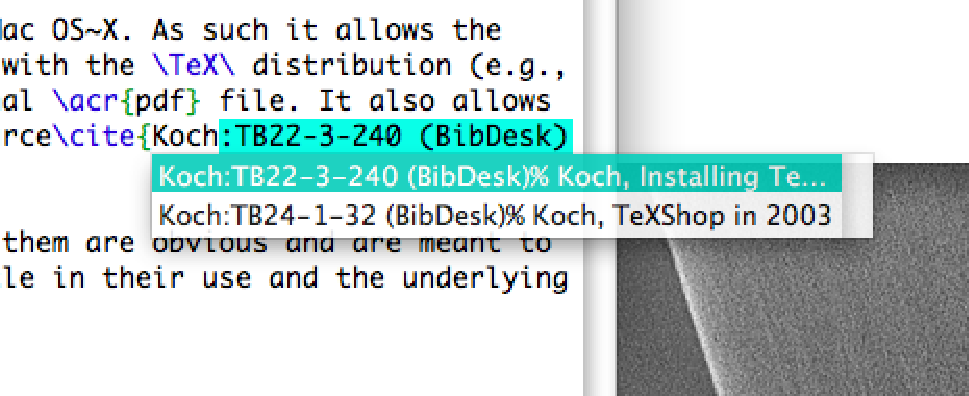
\includegraphics[width=2.7in]{figs/BibDeskPlugin}}\qquad\fbox{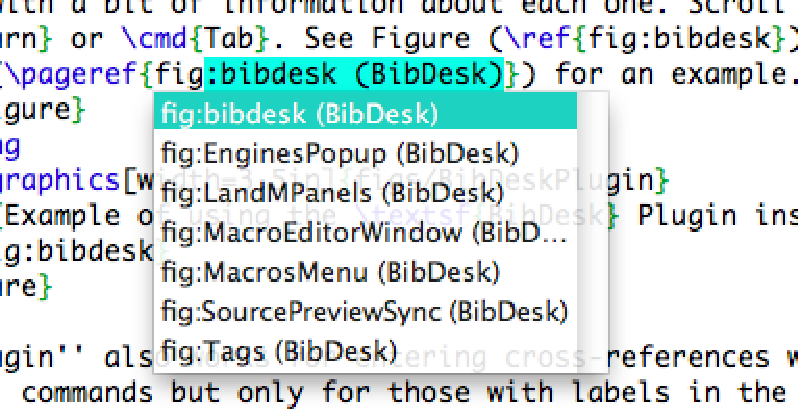
\includegraphics[height=1.2in]{figs/BibDeskPluginXref}}
\caption{Examples of using the \textsf{BibDesk} Plugin for citations and cross-references inside \TS.}
\label{fig:bibdesk}
\end{figure}

The ``plugin'' also works for entering cross-references within \verb|\ref| or \verb|\pageref| commands but only for those with labels in the file you are editing.

\subsection{Getting Help for Packages}

There are many times when having help about a given package can be handy. \TS\ has an interface to \texttt{texdoc} which will bring up that documentation. Execute the \mnu{Help}\To\mnu{Show Help for Package…} (\cmd{Opt-Cmd-I}) and enter the name of the package.

You can also easily look at a package directly with the \mnu{Help}\To\mnu{Open Style File…} command and enter the full package file name \emph{including the proper extension} (e.g., \texttt{.sty} for packages or \texttt{.cls} for document classes).

% Keyboard Shortcuts
%	For Menu Items via System Preferences->Keyboard & Mouse->Keyboard Shortcuts
%	For built-in frameworks via ~/Library/KeyBindings/DefaultKeyBinding.dict
%	Via editing MainMenu.nib
\section{Controlling the Keyboard}

One of the best ways to speed up your entry of text in a source file is to keep your hands on the keyboard as much as possible---only one of the reasons I don't like the ``clicky'' interface of the \LaTeX\ and Matrix Panels. There are many shortcuts associated with the \TS\ menu system but this section is about changing and adding others and other keyboard customizations.

\subsection{Menu Shortcuts \& System Preferences}

Sometimes you'd like to add a shortcut to a menu item that doesn't have one or add one to a command whose shortcut you dislike. Mac~OS~X 10.4 (Tiger) and later have a method to add shortcuts to specific menu items both globally and in specific programs. This feature has become much more reliable in OS~X~10.5 and especially in OS~X~10.6.

One example using Mac~OS~X~10.6 (Snow Leopard): \TS\ 2.36 has added a \mnu{File}\To\mnu{New from Stationery…} command, without a shortcut, which can be very helpful once you set up stationery the way you want. To add \cmd{Opt-Cmd-N} as the shortcut to that menu item: open up the \textsf{System Preferences} application to \mnu{Keyboard}\To\mnu{Keyboard Shortcuts} and select \mnu{Application Shortcuts}; press the \mnu{+} button to add a shortcut; select \TS\ as the application; enter the exact menu title [\mnu{New from Stationery…} --- note you \emph{must} enter a real ellipsis, `…', (\cmd{Opt-;} with the English keyboard layout)]; and press \cmd{Opt-Cmd-N} as the shortcut.

\subsection{More Editing Help}

\TS\ is built using Apple's programmers interfaces (called frameworks) and therefore inherits all the properties and functionality of those interfaces. There are many things available through the Text framework that aren't tied to the keyboard by default, e.g., many `\cmd{emacs}-like' keyboard commands, but Apple has made it possible to add those commands to all applications that use the Text framework; e.g., \textsf{TextEdit} and \textsf{Mail} as well as \TS.

This is done by creating a special file, \path{DefaultKeyBinding.dict}, and placing it in a particular location, \path{~/Library/KeyBindings/} (you may have to create the \path{KeyBindings} folder there if it doesn't already exist).

You can get more information about this, as well as a (useful) sample, by downloading the \path{KeyBindings.zip} file from <\url{http://public.me.com/herbs2}>.

%\subsection{What is Broken}

% Key Bindings (auto-completion)
%	via ~/Library/TeXShop/Keyboard/autocompletion.plist
\subsection{Key Bindings}

Besides adding shortcuts to Menu Items you can actually bind keystrokes, within \TS, to expand into groups of characters. Checking the \mnu{TeXShop}\To\mnu{Preferences}\To\mnu{Source}\To\mnu{Editor}\To\mnu{Key Bindings} option will enable this feature. You can also toggle it on/off for any particular document using \mnu{Source}\To\mnu{Key Bindings}\To\mnu{Toggle On/Off}. This feature was previously called Auto Completion; not to be confused with Command Completion---see section (\ref{sec:CC}) below.

E.g., pressing \cmd{Opt-,} with a US keyboard layout, usually enters \texttt{\(\leq\)} into your document but with Key Binding enabled \verb|\leq| will be entered. Similarly, with some text selected pressing \verb|"| will surround the selected text with \verb|``| and \verb|''|.

You can add, remove or change the key bindings using the Key Bindings Editor (\mnu{Source}\To\mnu{Key Bindings}\To\mnu{Edit Key Bindings File…}). Figures (\ref{fig:keybindingmenu}) and (\ref{fig:keybindeditor}) show the \mnu{Key Bindings} Menu and Editor.
\begin{figure}
\centering
\fbox{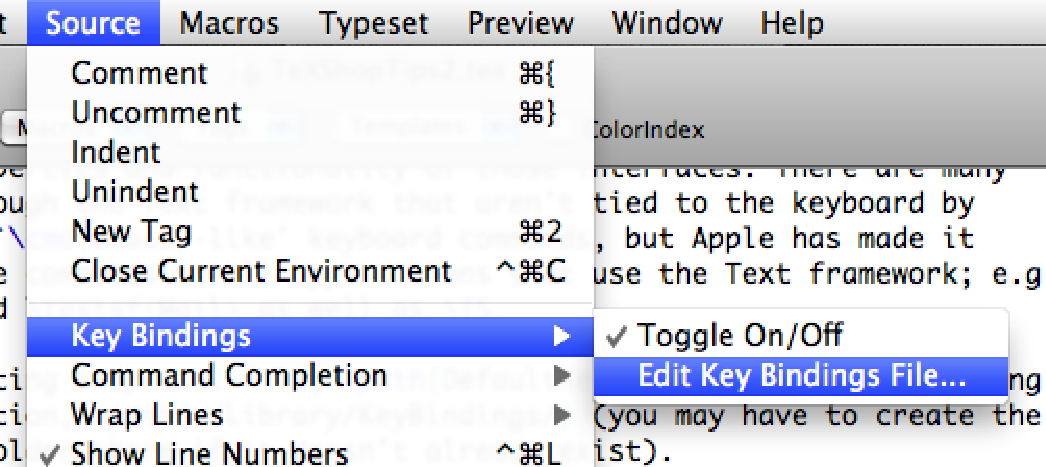
\includegraphics[width=3in]{figs/KeyBindingMenu}}
\caption{The Key Bindings Menu in \TS.}
\label{fig:keybindingmenu}
\end{figure}
\begin{figure}
\centering
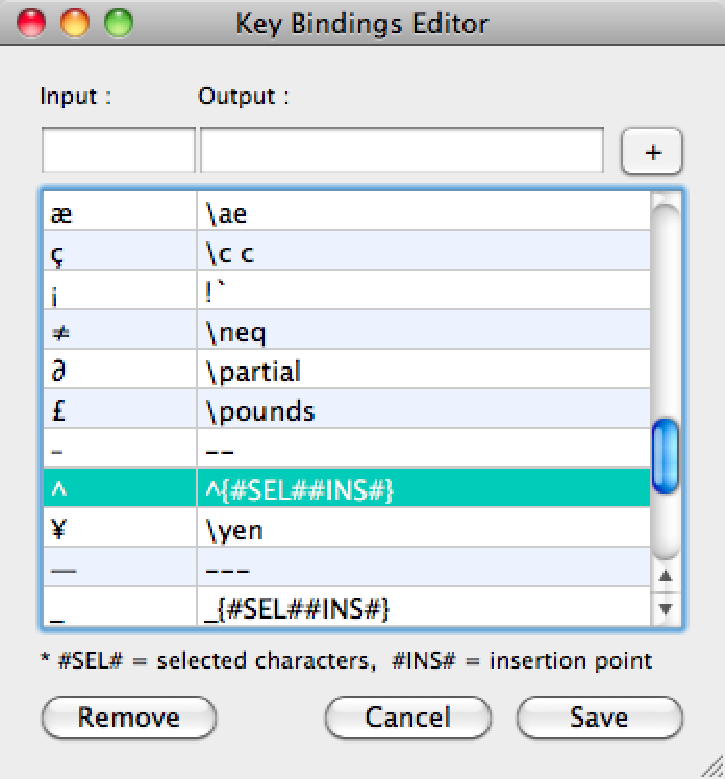
\includegraphics[height=2.00in]{figs/KeyBindingEditor}
\caption{The Key Bindings Editor in \TS.}
\label{fig:keybindeditor}
\end{figure}

%You can add your own keybindings and/or remove those you don't need by editing \path{~/Library/TeXShop/Keyboard/autocompletion.plist}. To add a keybinding to the \verb|_| key so that pressing it with a selection will produce the selection surrounded by \verb|_{| and \verb|}| enter the lines
%\begin{verbatim}
%	<key>_</key>
%	<string>_{#SEL##INS#}</string>
%\end{verbatim}
%to the list in \path{autocompetion.plist}.

% Macros
%	Applescript and Text macros and the Macros Menu
\section{Macros}

Macros can be simple text substitutions or Applescript programs that can do all sorts of processing on a file. You can also assign a keyboard shortcut to any macro for direct execution. The ones that are part of \TS\ are found under the \mnu{Macros} Menu.

You can remove or add additional macros to the menu by using the \mnu{Macro Editor} (use the \mnu{Macros}\To\mnu{Open Macro Editor} command). The \mnu{Macro Editor} window and extra menu items in the \mnu{Macros} Menu are shown in Figures (\ref{fig:MacroEditorWindow}) and (\ref{fig:MacrosMenu}) respectively.
\begin{figure}
\centering
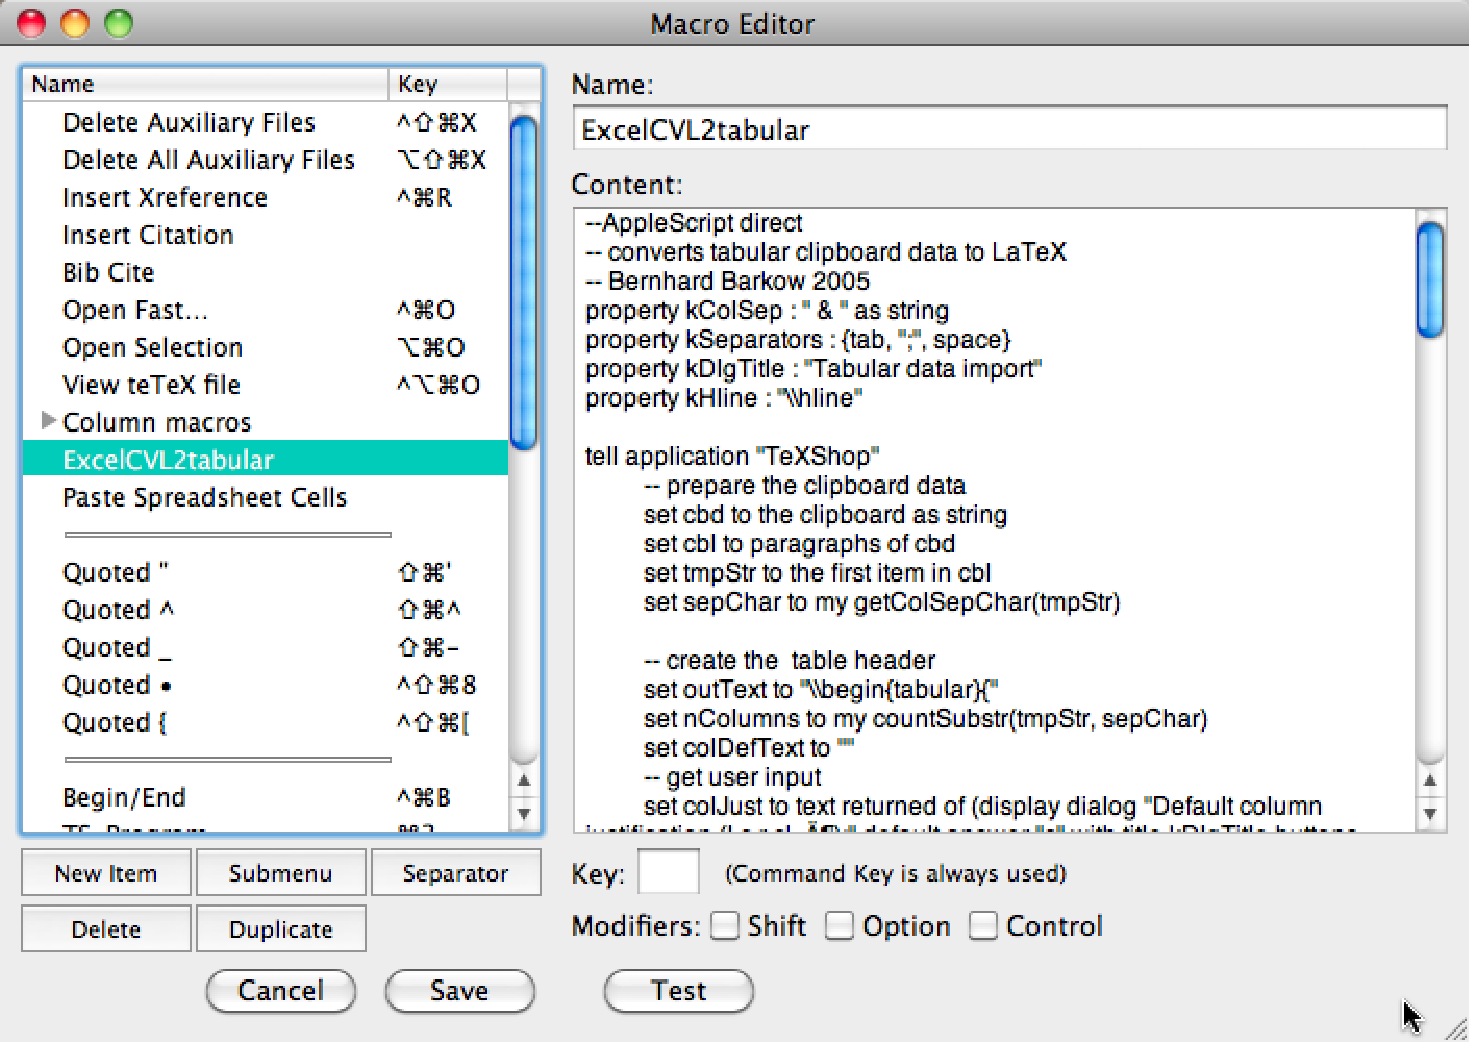
\includegraphics[width=4.75in]{figs/MacroEditorWindow}
\caption{The Macro Editor Window.}
\label{fig:MacroEditorWindow}
\end{figure}

Besides writing your own macros you can add macros supplied by others to the \mnu{Macros} menu one of two ways: copy and paste the text version of the macro into a \mnu{New Item} in the \mnu{Macro Editor}; or obtain the macro as a \texttt{plist} file and use the \mnu{Add macros from file…} command found in the \mnu{Macros} Menu when the \mnu{Macro Editor} is open (again, see Figure (\ref{fig:MacrosMenu})).
%\begin{figure}
%\centering
%\framebox{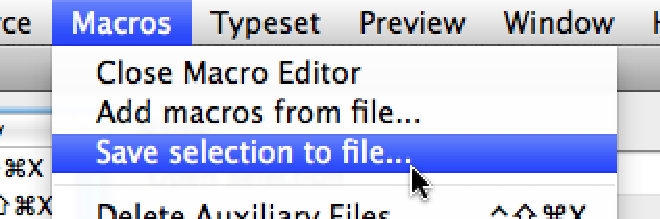
\includegraphics[width=2.5in]{figs/MacrosMenu}}
%\caption{The extra menu items when the Macro Editor is open.}
%\label{fig:MacrosMenu}
%\end{figure}

More information on macros can be found by searching for \cmd{macros} in \mnu{Help}\To\mnu{TeXShop Help Panel…}.

\subsection{Text Macros}

Text macros are simple text substitutions. You can also tell \TS\ to insert any selected text using \verb|#SEL#|, place the cursor using \verb|#INS#| and even put in multiple lines in the macro itself. Then you can assign the text macro to a keyboard shortcut.

I like to use \cmd{Cmd-B} and \cmd{Cmd-I} to insert \verb|\textbf{…}| and \verb|\emph{…}| into the document where \texttt{…} is any possible selected text. Macros to do that are already under the \mnu{Macros}\To\mnu{Text Styles} Menu so we need only assign keyboard shortcuts to them. To assign \cmd{Cmd-I} to the \mnu{emphasize} macro: open the \mnu{Macro Editor} where the form of the \mnu{Macros} menu appears in the left hand pane; click the \mnu{emphasize} macro found under \mnu{Text Styles}; click the Key insertion box and simply insert a lower case `\texttt{i}' (the \cmd{Cmd} key is assumed and additional modifier keys can be checked off).

\subsection{Applescript Macros}

You cannot distinguish Applescript macros in the \mnu{Macros} Menu from text macros but they can do complicated processing and add/change the source file in \TS. One example in the default set is the \mnu{Program} macro that creates a
\begin{verbatim}
% !TEX TS-program = xxxx
\end{verbatim}
line at the top of a file with your choice of engine substituted for \texttt{xxxx}. You can look at the Applescript code for this macro by clicking on its name in the \mnu{Macro Editor}.

\begin{figure}
\centering
\framebox{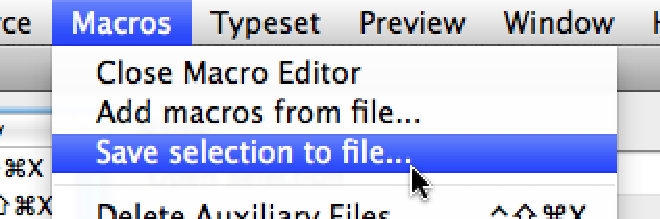
\includegraphics[width=2.25in]{figs/MacrosMenu}}
\caption{The extra menu items when the Macro Editor is open.}
\label{fig:MacrosMenu}
\end{figure}

% Command Completion
%	via ~/Library/TeXShop/CommandCompletion.txt & Macros
\section{Command Completion}\label{sec:CC}

\LaTeX\ markup is rather wordy which is nice because it describes what it's supposed to do but a bit painful to write. Command Completion allows you to insert complete environments and commands with a few keystrokes and the press of a ``trigger'' key (this is \cmd{Esc} by default but can be changed to \cmd{Tab} in \mnu{TeXShop}\To\mnu{Preferences}\To\mnu{Source}\To\mnu{Command Completion Triggered By:}).

Commands that have arguments usually have a Mark (\texttt{•}) inserted for each argument. You move to the next argument by using the \mnu{Source}\To\mnu{Command Completion}\To\mnu{Marks}\To\mnu{Next Mark} command (\cmd{Ctl-Cmd-F} [or \cmd{Opt-Trigger}]). This also selects the Mark so typing automatically removes the Mark and substitutes the typed information. See the complete documentation, with lists of commands/abbreviations supplied with \TS\ out of the box, in the \path{~/Library/TeXShop/CommandCompletion/} folder for much more information.

\subsection{Completions}

You can complete many commands by starting to type them and pressing the trigger key. Variations on the commands with differing numbers of optional arguments are generated by additional presses of the trigger. One example: typing \verb|\sec| and then the trigger on a new line produces
\begin{verbatim}
\section{|selmark}
\end{verbatim}
while a second press of the trigger gives
\begin{verbatim}
\section*{|selmark}
\end{verbatim}
the *-variant of the command and a final press of the trigger gives
\begin{verbatim}
\section[|selmark]{•}
\end{verbatim}
with the optional argument.

\subsection{Substitutions or Abbreviations}

Besides completions for partial command insertions there are also many abbreviations. These are short mnemonics for complete substitutions. 

All abbreviations for environments start with a `\texttt{b}'. To generate a complete \cmd{itemize} environment place \verb|\bite| on a line by itself and press the trigger key to get
\begin{verbatim}
\begin{itemize}
\item
|selmark
\end{itemize}•
\end{verbatim}
with an extra Mark at the end so you can easily jump to the end of the environment. Additional items can be generated by typing \verb|\it| and the trigger to get
\begin{verbatim}
\item
|selmark
\end{verbatim}
ready for entry of text.

In addition to the \verb|\section| command lower level sectioning commands have abbreviations. Sub-sections can be generated by typing \verb|\ssec| and the trigger to get
\begin{verbatim}
\subsection{|selmark}
\end{verbatim}
with subsequent presses of the trigger key giving the *-variant and finally the variant with the optional argument.

As a final example \verb|\tt| and the trigger gives the \verb|\texttt{|\selmark\verb|}| command and a second press of the trigger gives the declaration \verb|\ttfamily| with similar results for other font changing commands.

\subsection{Hey, it doesn't work!}

If these examples don't work you probably need to let \TS\ update the \path{~/Library/TeXShop/CommandCompletion/} folder; simply delete that folder from \path{~/Library/TeXShop/} and restart \TS.

% Engines
%	via ~/Library/TeXShop/Engines/
\section{Extending Processing via Engines}

\TS\ offers several default ``engines'' (also referred to as ``scripts'' which is left over from earlier times) in its \mnu{Typeset} Menu. These include running \mnu{Plain TeX} or \mnu{LaTeX} (either using \texttt{pdftex} or \texttt{TeX+DVI}), \mnu{BibTeX}, \mnu{MakeIndex}, \mnu{MetaPost} or \mnu{ConTeXt}. But there are many things you may wish to do that fall outside of this limited set so \TS\ also allows you to create new engines that are stored in \path{~/Library/TeXShop/Engines/}. These additional engines do not show up in the \mnu{Typeset} menu but only in the popup list on the Source and Preview Toolbar (see Figure (\ref{fig:EnginesPopup})). 

You can use these engines by choosing from that popup list and then pressing the Typeset button or, a better choice if you use different engines for different documents, by putting a line like
\begin{verbatim}
% !TEX TS-program = xelatex
\end{verbatim}
at the top of your source file; the example given will run the \texttt{xelatex} engine on this file independent of other choices.

\TS\ is shipped with a few engines activated (i.e., directly in the \path{~/Library/TeXShop/Engines/} folder) but also includes several additional ones in \path{~/Library/TeXShop/Engines/Inactive/}. As an example let's activate and use the \cmd{pdflatexmk} engine found in \path{~/Library/TeXShop/Engines/Inactive/Latexmk/}.
\begin{figure}
\centering
\framebox{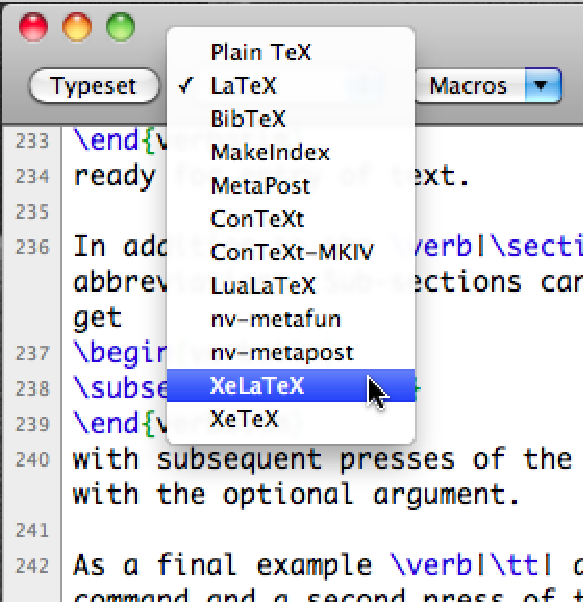
\includegraphics[width=2.0in]{figs/EnginesPopup}}
\caption{The Engines Popup Menu on the Source Toolbar.}
\label{fig:EnginesPopup}
\end{figure}

\subsection{The \texttt{pdflatexmk} engine}

If your document had cross-references, bibliographies or indexes it takes multiple \texttt{pdflatex} runs with intermediate runs of \texttt{bibtex} and/or \texttt{makeindex} to create the bibliographies, indexes and resolve all cross-references. The \texttt{pdflatexmk} engine automates this whole process.

To activate the engine simply move the \texttt{pdflatexmk.engine} file from \path{~/Library/TeXShop/Engines/Inactive/Latexmk/} two folders up, to \path{~/Library/TeXShop/Engines/}. When you restart \TS\ you can check that \cmd{pdflatexmk} in now in the popup menu.

Now place the line
\begin{verbatim}
% !TEX TS-program = pdflatexmk
\end{verbatim}
at the top of your source file. From then on when you simply typeset the file (\mnu{Typeset}\To\mnu{Typeset} or \cmd{Cmd-T}) \TS\ will use this engine and the complete process for typesetting the document to its final form will be carried out.

\end{document}
